%!TEX root = informe.tex
\chapter{Análisis de Ciclo de Vida de un adoquín: evaluación del impacto ambiental (EICV) e interpretación}

\section{Introducción}
La norma UNE–EN-ISO 14040:2006 \cite{iso14040} indica que ``la fase de EICV es para conocer y evaluar la magnitud y cuán significativos son los impactos potenciales ambientales de un sistema del producto a través de todo el ciclo de vida del producto''.

En esta etapa, se utilizan los datos recopilados en la fase de Inventario ICV vistos en el capítulo \ref{cap:inventario} y se hace un enfoque relativo del impacto ambiental basado en la Unidad Funcional, convirtiendo los datos del ICV a unidades comunes, sumando posteriormente los resultados obtenidos dentro de la misma categoría de impacto, siguiendo la metodología explicada en la sección \ref{sec:metodologiaeicv}.

En este proyecto también se desarrollarán las etapas opcionales de normalización, agrupación y ponderación de los resultados.

Como se ha establecido la sección \ref{sec:categoriasimpactoseleccionadas}, para la elección de las categorías de impacto, el método ReCiPe recoge 21 categorías, de las cuales se ha seleccionado las más significativas mediante una previsualización de los resultados:

\begin{itemize}
  \item Cambio climático — Salud humana (CC[HH]).
  \item Toxicidad humana (HT).
  \item Formación de partículas (PMF).
  \item Cambio climático - Ecosistemas (CC[Ec]).
  \item Agotamiento de recursos fósiles (FD).
\end{itemize}

Una vez introducidos los datos del inventario para todas las fases del ciclo de vida del producto en el software de análisis SimaPro, se aplica el método de análisis \textit{ReCiPe Endpoint (H) V1.06 / Europe ReCipe H/A}, desarrollado en la sección \ref{sec:recipe}.

\section{Evaluación del Impacto Ambiental de la fase de extracción de materias primas, fabricación e instalación}

La red de la fase de extracción de materias primas, fabricación e instalación de la figura \ref{fig:fabric_red} se muestran todos los procesos interrelacionados para dar una perspectiva general de la fase.

\begin{figure}[!htb]
\centering
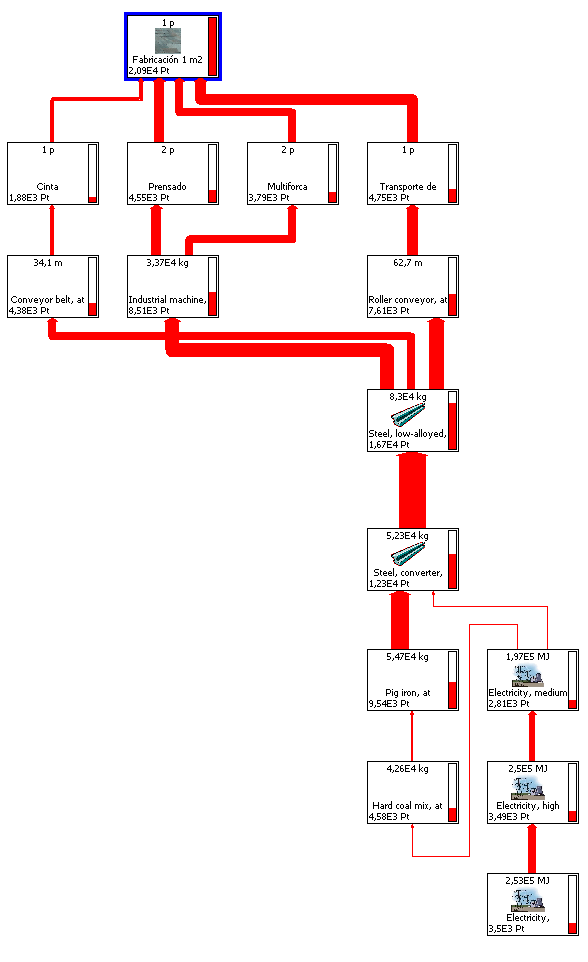
\includegraphics[height=15cm]{img/fabric_red.png}
\caption{Red de la fase de extracción de materias primas, fabricación e instalación.}
\label{fig:fabric_red}
\end{figure}

Cada caja gris representa un proceso y cada proceso se muestra una única vez. Las cajas azul de color azul representan ensamblajes. Las flechas representan los flujos entre procesos. Las barras rojas o termómetros indican la carga medioambiental generada en cada proceso y sus procesos aguas arriba. De esta manera se puede distinguir entre los procesos más importantes y los menos, identificando los puntos calientes.

De la red de la fase de extracción de materias primas, fabricación e instalación se puede obtener los transportadores de rodillo, cintas transportadoras, prensas y multiforcas son los procesos con mayor carga medioambiental de esta fase.

La caracterización del análisis de impacto muestra todas las categorías de impacto. Cada una de ellas tiene una unidad de medida diferente, por lo que se representan gráficamente de forma porcentual. Para tener una visión más clara de los impactos relevantes de la fase, es mejor recurrir a la normalización donde las diferentes puntuaciones de los impactos caracterizados se relativizan a una referencia común.

La figura \ref{fig:fabric_normalizacion} y la tabla \ref{categoriasimpactofabricacion} muestran las categorías de impacto relevantes de esta fase.

\begin{figure}[!htb]
\centering
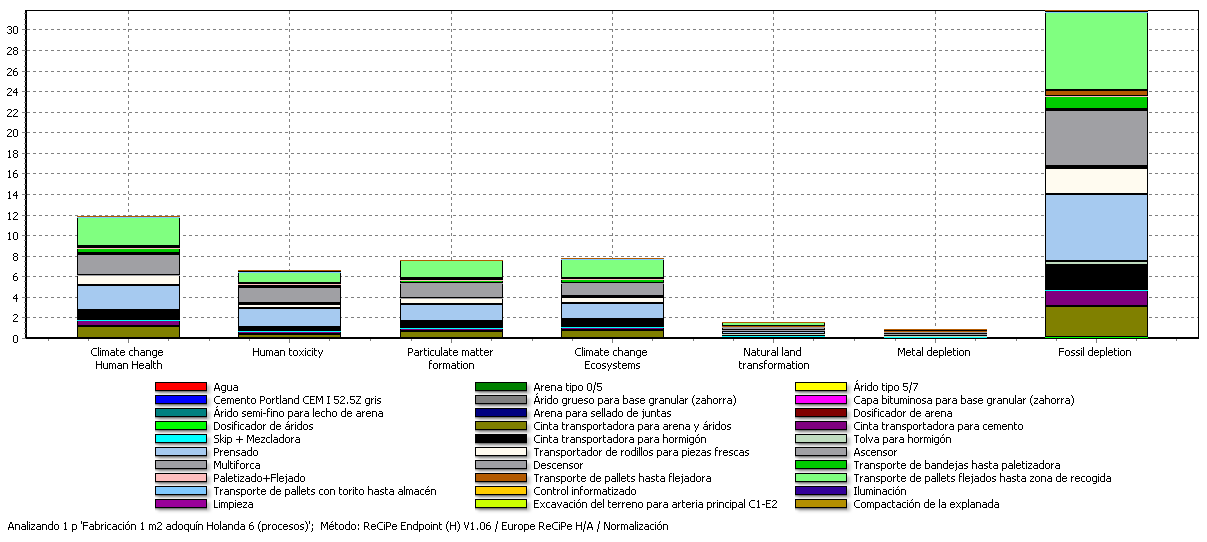
\includegraphics[width=15cm]{img/fabric_normalizacion.png}
\caption{Cuantificación de los impactos normalizados de la fase de extracción de materias primas, fabricación e instalación.}
\label{fig:fabric_normalizacion}
\end{figure}

La categoría con mayor impacto es la de ``Agotamiento de recursos fósiles'', donde destacan el transporte de pallets flejados hasta la zona de recogida, la multiforca y el prensado. Para el resto de categorías de impacto se produce una situación similar.

\begin{table}[!htb]
\centering
\begin{tabular}{p{4cm}rrrrr}
\toprule
\multicolumn{6}{c}{Categorías de impacto}\\
\midrule
Proceso & CC[HH] & HT & FMP & CC[Ec] & FD\\
 &  (\%) & (\%) & (\%) & (\%) & (\%)\\
\midrule
Transporte de pallets flejados hasta la zona de recogida & 23.7 & 17.1 & 23 & 23.7 & 23.5\\
Multiforca & 16.9 & 24.2 & 18.4 & 16.9 & 17\\
Prensado & 20.3 & 29.1 & 22.1 & 20.3 & 20.4\\
\bottomrule
\end{tabular}
\caption[Categorías de impacto de la fase de extracción de materias primas, fabricación e instalación.]{Categorías de impacto de la fase de extracción de materias primas, fabricación e instalación. CC[HH]: cambio climático—salud humana, HT: toxicidad humana, FMP: formación de partículas, CC[Ec]: cambio climático—ecosistema, FD: agotamiento de recursos fósiles.}
\label{categoriasimpactofabricacion}
\end{table}

La puntuación única permite observar los resultados desde una perspectiva diferente. Esta opción agrupa las categorías de impacto aplicando una serie de puntos a cada una, representando finalmente todas las categorías de impacto usando una misma unidad, el Kilopunto (\textit{kiloPoint}, kPt). La carga ambiental será mayor cuanto más kPt tenga.

\begin{figure}[!htb]
\centering
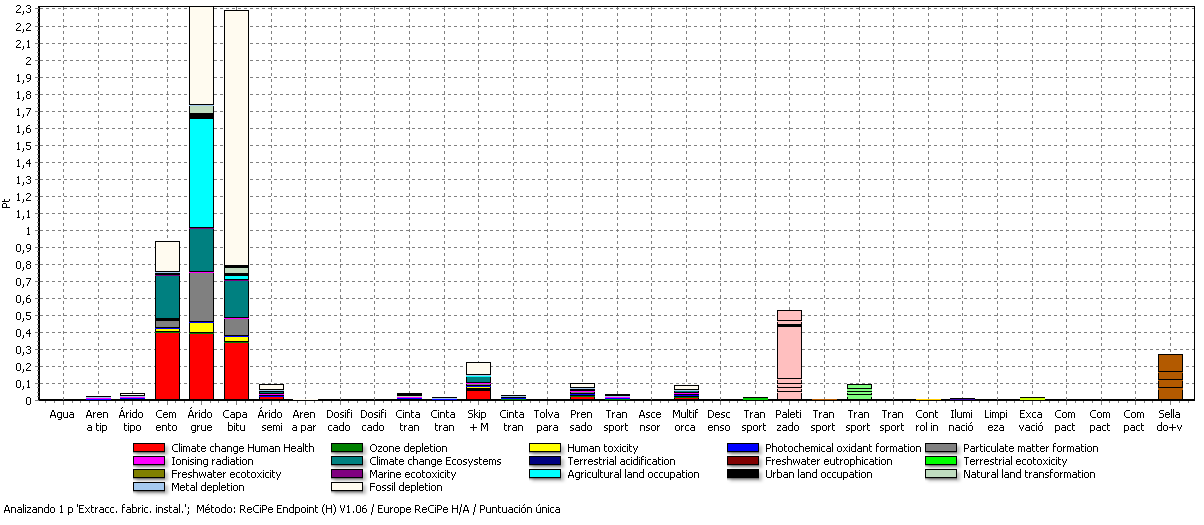
\includegraphics[width=15cm]{img/fabric_puntuacionunica.png}
\caption{Cuantificación de los impactos a nivel de puntuación única de la fase de extracción de materias primas, fabricación e instalación.}
\label{fig:fabric_puntuacionunica}
\end{figure}

La figura \ref{fig:fabric_puntuacionunica} muestra las categorías de impacto a nivel de puntuación única. Los resultados son similares a los de la normalización, donde el transporte de pallets flejados hasta la zona de recogida, la multiforca y el prensado tienen la mayor puntuación.

Atendiendo a las categorías de daños (punto final) de la tabla \ref{categoriasdanosfabricacion}, los resultados indican que el mayor daño se produce en la salud humana.

\begin{table}[!htb]
\centering
\begin{tabular}{p{6cm}rrr}
\toprule
\multicolumn{4}{c}{Categorías de daño}\\
\midrule
Proceso & Salud hum. & Ecosistema & Recursos\\
 & (kPt) & (kPt) &  (kPt)\\
\midrule
Transporte de pallets flejados hasta la zona de recogida & 4.75 & 0.94 & 1.53\\
Multiforca & 2 & 0.67 & 1.12\\
Prensado & 2.4 & 0.80 & 1.35\\
\midrule
Total (kPt) & 9.15 & 2.41 & 4.00\\
\bottomrule
\end{tabular}
\caption{Categorías de daños de la fase de extracción de materias primas, fabricación e instalación.}
\label{categoriasdanosfabricacion}
\end{table}

\section{Evaluación del Impacto Ambiental de la fase de uso y mantenimiento}

La red de la fase de uso y mantenimiento de la figura \ref{fig:uso_red} muestra todos los procesos interrelacionados para dar una perspectiva general de la fase.

\begin{figure}[!htb]
\centering
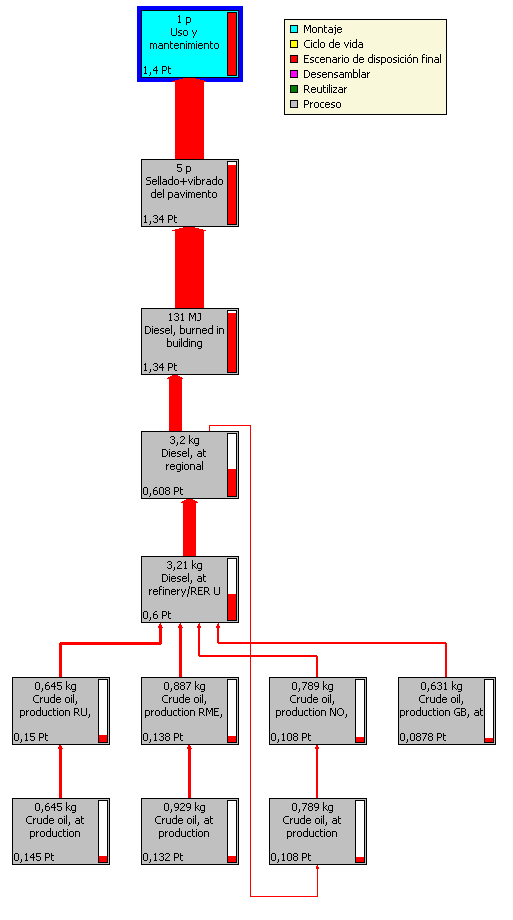
\includegraphics[height=15cm]{img/uso_red.png}
\caption{Red de la fase de uso y mantenimiento.}
\label{fig:uso_red}
\end{figure}

Cada caja gris representa un proceso y cada proceso se muestra una única vez. Las cajas azul de color azul representan ensamblajes. Las flechas representan los flujos entre procesos. Las barras rojas o termómetros indican la carga medioambiental generada en cada proceso y sus procesos aguas arriba. De esta manera se puede distinguir entre los procesos más importantes y los menos, identificando los puntos calientes.

Como era de esperar, en la red de la fase de uso y mantenimiento el proceso con mayor carga ambiental es el sellado y vibrado del pavimento.

La caracterización del análisis de impacto muestra todas las categorías de impacto. Cada una de ellas tiene una unidad de medida diferente, por lo que se representan gráficamente de forma porcentual. Para tener una visión más clara de los impactos relevantes de la fase, es mejor recurrir a la normalización donde las diferentes puntuaciones de los impactos caracterizados se relativizan a una referencia común.

La figura \ref{fig:uso_normalizacion} y la tabla \ref{categoriasimpactouso} muestran las categorías de impacto relevantes de esta fase.

\begin{figure}[!htb]
\centering
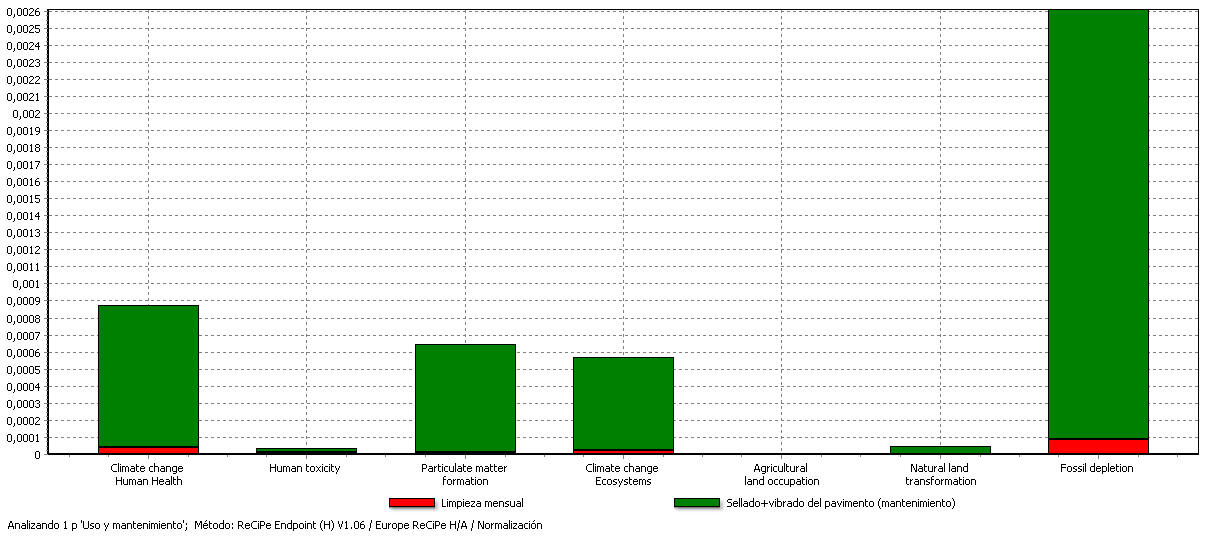
\includegraphics[width=15cm]{img/uso_normalizacion.png}
\caption{Cuantificación de los impactos normalizados de la fase de uso y mantenimiento.}
\label{fig:uso_normalizacion}
\end{figure}

Al igual que en la fase de extracción de materias primas, fabricación e instalación, la categoría con mayor impacto es la de ``Agotamiento de recursos fósiles'', donde el sellado y vibrado del pavimento es el proceso dominante. El resto de categorías de impacto muestran la misma situación.

\begin{table}[!htb]
\centering
\begin{tabular}{p{4cm}rrrrr}
\toprule
\multicolumn{6}{c}{Categorías de impacto}\\
\midrule
Proceso & CC[HH] & HT & FMP & CC[Ec] & FD\\
 &  (\%) & (\%) & (\%) & (\%) & (\%)\\
\midrule
Sellado y vibrado & 95.5 & 61.4 & 98.2 & 95.5 & 96.5\\
\bottomrule
\end{tabular}
\caption[Categorías de impacto de la fase de uso y mantenimiento.]{Categorías de impacto de la fase de uso y mantenimiento. CC[HH]: cambio climático—salud humana, HT: toxicidad humana, FMP: formación de partículas, CC[Ec]: cambio climático—ecosistema, FD: agotamiento de recursos fósiles.}
\label{categoriasimpactouso}
\end{table}

La puntuación única permite observar los resultados desde una perspectiva diferente. Esta opción agrupa las categorías de impacto aplicando una serie de puntos a cada una, representando finalmente todas las categorías de impacto usando una misma unidad, el Kilopunto (\textit{kiloPoint}, kPt). La carga ambiental será mayor cuanto más kPt tenga.

\begin{figure}[!htb]
\centering
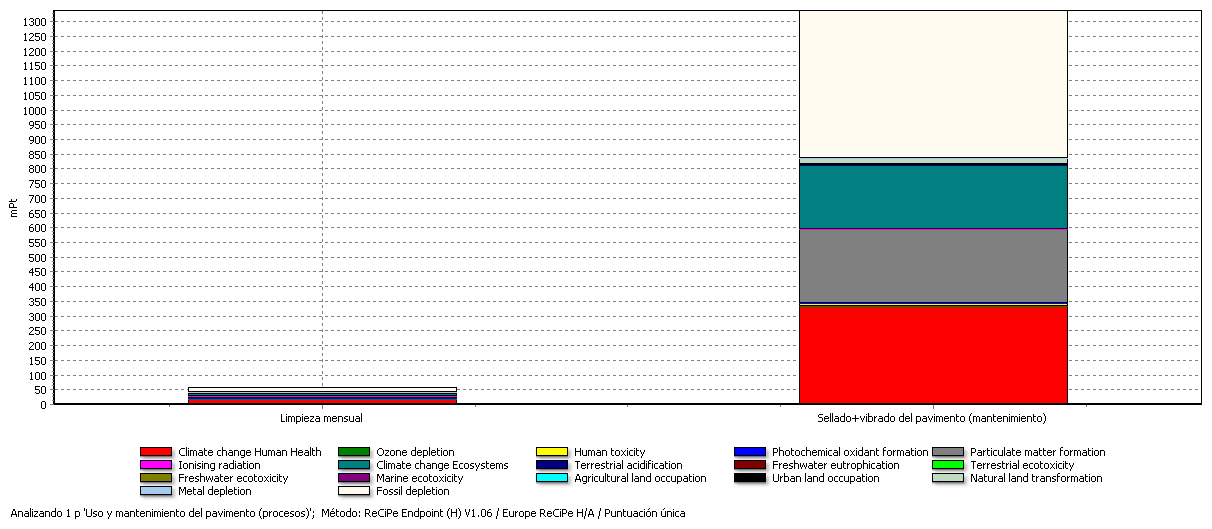
\includegraphics[width=15cm]{img/uso_puntuacionunica.png}
\caption{Cuantificación de los impactos a nivel de puntuación única de uso y mantenimiento.}
\label{fig:uso_puntuacionunica}
\end{figure}

La figura \ref{fig:uso_puntuacionunica} muestra las categorías de impacto a nivel de puntuación única. Los resultados son similares a los de la normalización. El proceso de sellado y vibrado del pavimento afecta principalmente a las categorías de agotamiento de recursos fósiles y al cambio climático desde el punto de vista de la salud humana. El menor medida afecta al cambio climática visto desde el ecosistema y a la formación de partículas.

Atendiendo a las categorías de daños (punto final) de la tabla \ref{categoriasdanosuso}, los resultados indican que el mayor daño se produce en la salud humana.

\begin{table}[!htb]
\centering
\begin{tabular}{p{6cm}rrr}
\toprule
\multicolumn{4}{c}{Categorías de daño}\\
\midrule
Proceso & Salud hum. & Ecosistema & Recursos\\
& (kPt) &  (kPt) &  (kPt)\\
\midrule
Vibrado y sellado & 0.59 & 0.24 & 0.50\\
\bottomrule
\end{tabular}
\caption{Categorías de daños de la fase de uso y mantenimiento.}
\label{categoriasdanosuso}
\end{table}

\section{Evaluación del Impacto Ambiental de la fase de fin de vida}

En la red de la fase de fin de vida de la figura \ref{fig:fdv_red} se muestran todos los procesos interrelacionados para dar una perspectiva general de la fase.

\begin{figure}[!htb]
\centering
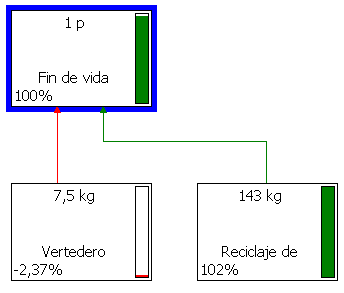
\includegraphics[height=15cm]{img/fdv_red.png}
\caption{Red de la fase de fin de vida.}
\label{fig:fdv_red}
\end{figure}

Cada caja gris representa un proceso y cada proceso se muestra una única vez. Las cajas azul de color azul representan ensamblajes. Las flechas representan los flujos entre procesos. Las barras rojas o termómetros indican la carga medioambiental generada en cada proceso y sus procesos aguas arriba. De esta manera se puede distinguir entre los procesos más importantes y los menos, identificando los puntos calientes.

En la red de la fase de fin de vida el proceso con mayor carga ambiental es el reciclaje del adoquín en árido, como era de esperar.

La caracterización del análisis de impacto muestra todas las categorías de impacto. Cada una de ellas tiene una unidad de medida diferente, por lo que se representan gráficamente de forma porcentual. Para tener una visión más clara de los impactos relevantes de la fase, es mejor recurrir a la normalización donde las diferentes puntuaciones de los impactos caracterizados se relativizan a una referencia común.

La figura \ref{fig:fdv_normalizacion} y la tabla \ref{categoriasimpactofdv} muestran las categorías de impacto relevantes de esta fase.

\begin{figure}[!htb]
\centering
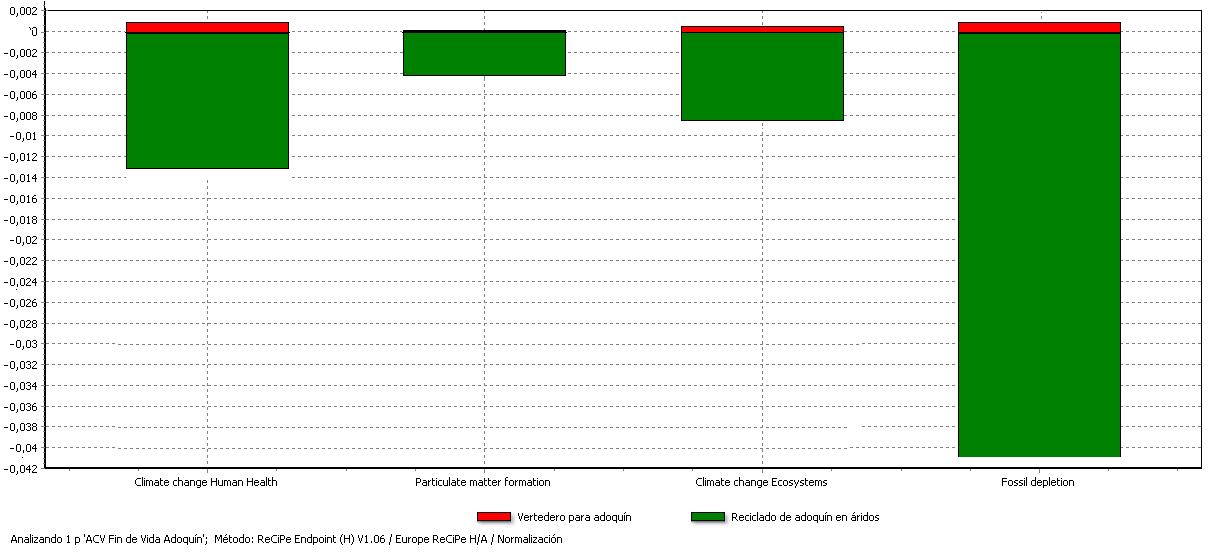
\includegraphics[width=15cm]{img/fdv_normalizacion.png}
\caption{Cuantificación de los impactos normalizados de la fase de fin de vida.}
\label{fig:fdv_normalizacion}
\end{figure}

Al igual que en las dos fases anteriores, la categoría con mayor impacto es la de ``Agotamiento de recursos fósiles'', donde el reciclaje de adoquín en árido es el proceso que más afecta a todas las categorías de impacto.

\begin{table}[!htb]
\centering
\begin{tabular}{p{4cm}rrrrr}
\toprule
\multicolumn{6}{c}{Categorías de impacto}\\
\midrule
Proceso & CC[HH] & HT & FMP & CC[Ec] & FD\\
 & (\%) & (\%) & (\%) & (\%) & (\%)\\
\midrule
Reciclaje de adoquín en árido & -92.6 & -92.7 & -96.7 & -92.6 & -97.6\\
\bottomrule
\end{tabular}
\caption[Categorías de impacto de la fase de fin de vida.]{Categorías de impacto de la fase de fin de vida. CC[HH]: cambio climático—salud humana, HT: toxicidad humana, FMP: formación de partículas, CC[Ec]: cambio climático—ecosistema, FD: agotamiento de recursos fósiles.}
\label{categoriasimpactofdv}
\end{table}

La puntuación única permite observar los resultados desde una perspectiva diferente. Esta opción agrupa las categorías de impacto aplicando una serie de puntos a cada una, representando finalmente todas las categorías de impacto usando una misma unidad, el Kilopunto (\textit{kiloPoint}, kPt). La carga ambiental será mayor cuanto más kPt tenga.

\begin{figure}[!htb]
\centering
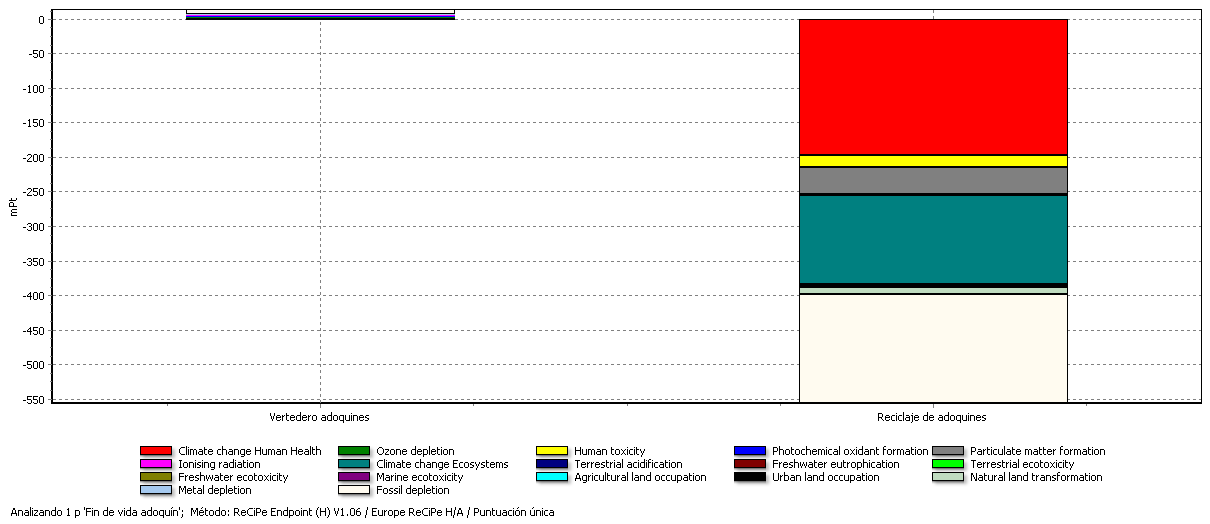
\includegraphics[width=15cm]{img/fdv_puntuacionunica.png}
\caption{Cuantificación de los impactos a nivel de puntuación única de fin de vida.}
\label{fig:fdv_puntuacionunica}
\end{figure}

La figura \ref{fig:fdv_puntuacionunica} muestra las categorías de impacto a nivel de puntuación única. Los resultados son similares a los de la normalización y a las otras fases del ciclo de vida. El proceso de reciclaje de adoquín en áridos afecta principalmente a las categorías de agotamiento de recursos fósiles y al cambio climático desde el punto de vista de la salud humana. También afecta en menor proporción al cambio climática visto desde el ecosistema y a la formación de partículas.

Atendiendo a las categorías de daños (punto final) de la tabla \ref{categoriasdanosfdv}, los resultados indican que el mayor daño en esta fase se produce en los recursos.

\begin{table}[!htb]
\centering
\begin{tabular}{p{6cm}rrr}
\toprule
\multicolumn{4}{c}{Categorías de daño}\\
\midrule
Proceso & Salud hum. & Ecosistema & Recursos\\
 & (kPt) & (kPt) & (kPt)\\
\midrule
Reciclaje de adoquín en árido & -7.27 & -3.78 & -8.37\\
\bottomrule
\end{tabular}
\caption{Categorías de daños de la fase de fin de vida.}
\label{categoriasdanosfdv}
\end{table}

\section{Evaluación del Impacto Ambiental comparativo de todas las fases}

Una vez estudiadas las tres fases del ciclo de vida por separado es interesante hacer una comparación entre las tres etapas.

A priori, observando los resultados ya obtenidos en las tablas de categorías de impacto \ref{categoriasimpactofabricacion}, \ref{categoriasimpactouso} y \ref{categoriasimpactofdv}, se puede asegurar que las etapas de uso y mantenimiento y fin de vida apenas tienen consecuencias comparadas con la de extracción de materias primas, fabricación e instalación. Esto puede ratificar las características que tienen los pavimentos de adoquín (sección \ref{sec:ventajas}, donde el coste de fabricación es mayor, pero el mantenimiento y su reutilización hacen que sea una opción muy recomendable a largo plazo.

La categoría con mayor impacto es la de ``Agotamiento de recursos fósiles'', donde la fase que predomina es la de extracción de materias primas, fabricación e instalación en todas las categorías de impacto (ver figura \ref{fig:compar_normalizacion}).

\begin{figure}[!htb]
\centering
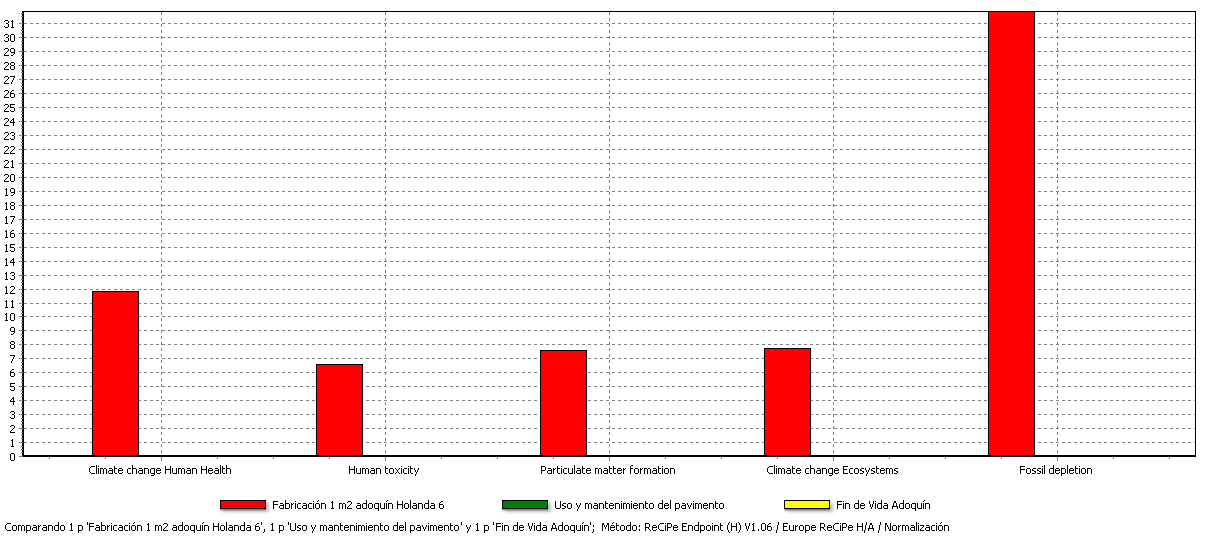
\includegraphics[width=15cm]{img/compar_normalizacion.png}
\caption{Cuantificación de los impactos normalizados comparativo entre las tres fases.}
\label{fig:compar_normalizacion}
\end{figure}

La tabla de categoría de daños \ref{categoriasdanoscompar} se puede extraer la conclusión de que la fase que más contribuye al perfil ambiental del adoquín es la de extracción de materias primas, fabricación e instalación.

\begin{table}[!htb]
\centering
\begin{tabular}{p{6cm}rrr}
\toprule
\multicolumn{4}{c}{Categorías de daño}\\
\midrule
Etapa & Salud hum. & Ecosistema & Recursos\\
 & (kPt) & (kPt) & (kPt)\\
\midrule
Extracc., fabric. e instal. & 26 & 9.86 & 32.7\\
Uso y mantenim. & 0.0016 & 0.0006 & 0.0026 \\
Fin de vida & -0.019 & -0.01 & -0.04 \\
\bottomrule
\end{tabular}
\caption{Categorías de daños de la comparación entre fases.}
\label{categoriasdanoscompar}
\end{table}

A continuación se realizará un análisis de con el método de cálculo de \textbf{Demanda de Energía Acumulada} para conocer la energía que se consume en esta fase. La figura \ref{fig:ced_puntuacionunica} y la tabla \ref{tiposenergiaced} muestran que existe el mayor consumo de energía se produce en la fase de extracción de materias primas, fabricación e instalación, y el tipo de energía consumida es fósil no renovable, un 83.4\% en esa fase. Las energías nuclear y renovables representan un 11.3\% y un 5.2\% respectivamente. Por tanto, es esta fase donde hay que mejorar el consumo y por tanto su perfil ambiental.


\begin{figure}[!htb]
\centering
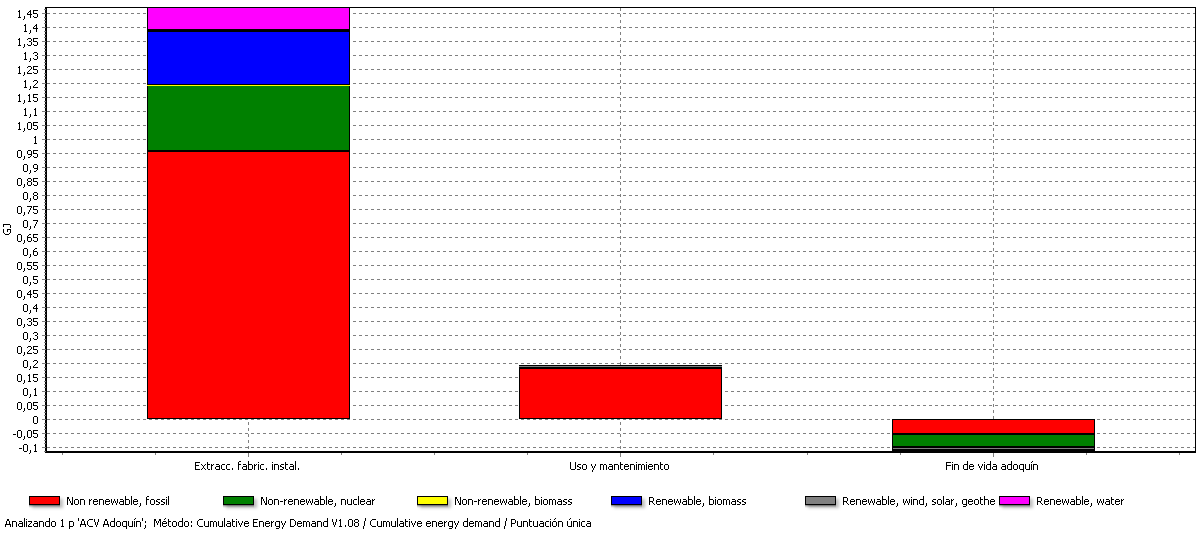
\includegraphics[width=15cm]{img/ced_puntuacionunica.png}
\caption{Cuantificación de los impactos a nivel de puntuación única CED comparativo entre las tres fases.}
\label{fig:ced_puntuacionunica}
\end{figure}

\begin{table}[!htb]
\centering
\begin{tabular}{p{2cm}rrrrrr}
\toprule
\multicolumn{7}{c}{Tipos de energía consumidos}\\
\midrule
 & \multicolumn{3}{c}{No renovables} & \multicolumn{3}{c}{Renovables}\\
\midrule
Etapa & Fósil & Nuclear & Biom. & Biom. & Viento, sol,& Agua\\
& (\%) & (\%) & (\%) & (\%) & geo (\%) & (\%)\\
\midrule
Extracc., fabric. e instal. & 83.4 0& 11.30 & 0.02 & 0.92 & 0.20 & 4.09\\
Uso y mantenim. & 95.40 & 3.71 & 0.01 & 0.40 & 0.70 & 0.47 \\
Fin de vida & -92.40 & -6.23 & -0.01 & -0.19 & -0.05 & -1.14 \\
\bottomrule
\end{tabular}
\caption{Tipos de energía consumidos en cada fase.}
\label{tiposenergiaced}
\end{table}

Finalmente, se utiliza el método IPCC para el cálculo potencial del calentamiento global a lo largo del ciclo de vida. Se aplicará un horizonte temporal a 100 años (GWP 100a) para conocer los kilogramos de \ce{CO2} equivalentes que genera el producto en base a su Unidad Funcional (ver tabla.

\begin{table}[!htb]
\centering
\begin{tabular}{p{6cm}r}
\toprule
\multicolumn{2}{c}{Generación de \ce{CO2}}\\
\midrule
Etapa & IPCC GWP 100a (\si{kg}\ce{CO2} eq.)\\
\midrule
Extracc., fabric. e instal. & 1.7E5\\
Uso y mantenim. & 12.5\\
Fin de vida & -203\\
\bottomrule
\end{tabular}
\caption{IPCC 2007 GWP 100a: kilogramos de $CO_2$ equivalente generados en cada fase.}
\label{co2generado}
\end{table}


